% =======================================================
% =======         HEADER FOR DOCUMENT        ============
% =======================================================
    
    % *********  SPECIFIC FOR THIS BOOK  ********
    \def\ProjectAuthorLink{https://github.com/SoyOscarRH}
    \def\ProjectNameLink{/}    
    

    % *********   DOCUMENT ITSELF   **************
    \documentclass[12pt, fleqn]{report}                             %Type of doc and size of font and left equations
    \usepackage[margin=1.2in]{geometry}                             %Margins and Geometry pacakge
    \usepackage{ifthen}                                             %Allow simple programming using if - then
    \usepackage[hidelinks]{hyperref}                                %Allow to create hiperlinks and Fuck Firefox
    \usepackage{pdfpages}                                           %Allow us 'import' PDF's
    \hypersetup{pageanchor=false}                                   %Solve 'double page 1' warnings in build :v
    \setlength{\parindent}{0pt}                                     %Eliminate ugly indentation
    \author{Oscar Andrés Rosas}                                     %Who I am

    \usepackage{subcaption}

    % *********   LANGUAJE    *****************
    \usepackage[spanish]{babel}                                     %Please allow me to type in spanish
    \usepackage[utf8]{inputenc}                                     %Lets use UFT-8
    \usepackage[T1]{fontenc}                                        %Allow for better font support
    \usepackage{textcmds}                                           %Allow us to use quoutes
    \usepackage{changepage}                                         %Allow us to use identate paragraphs
    \usepackage{anyfontsize}                                        %All the sizes for fonts wiiiii!

    % *********   MATH AND HIS STYLE  *********
    \usepackage{ntheorem, amsmath, amssymb, amsfonts}               %All fucking math, I want all!
    \usepackage{mathrsfs, mathtools, empheq}                        %All fucking math, I want all!
    \usepackage{cancel}                                             %Negate symbol
    \usepackage{centernot}                                          %Allow me to negate a symbol
    \decimalpoint                                                   %Use decimal point

    % *********   GRAPHICS AND IMAGES *********
    \usepackage{graphicx}                                           %Allow to create graphics
    \usepackage{float}                                              %For images
    \usepackage{wrapfig}                                            %Allow to create images
    \graphicspath{ {Graphics/} }                                    %Where are the images :D

    % *********   LISTS AND TABLES ***********
    \usepackage{listings, listingsutf8}                             %We will be using code here
    \usepackage[inline]{enumitem}                                   %We will need to enumarate
    \usepackage{tasks}                                              %Horizontal lists
    \usepackage{longtable}                                          %Lets make tables awesome
    \usepackage{booktabs}                                           %Lets make tables awesome
    \usepackage{tabularx}                                           %Lets make tables awesome
    \usepackage{multirow}                                           %Lets make tables awesome
    \usepackage{multicol}                                           %Create multicolumns

    % *********   REMOVE SOME ERRORS **********
    \hbadness=10000                                                 %Ignore \vbox and \hbox warings
    \hfuzz=\maxdimen\newdimen\hfuzz                                 %Ignore \vbox and \hbox warings

    % *********   HEADERS AND FOOTERS ********
    \usepackage{fancyhdr}                                           %Lets make awesome headers/footers
    \pagestyle{fancy}                                               %Lets make awesome headers/footers
    \setlength{\headheight}{16pt}                                   %Top line
    \setlength{\parskip}{0.5em}                                     %Top line
    \renewcommand{\footrulewidth}{0.5pt}                            %Bottom line

    \lhead {                                                        %Left Header
        \hyperlink{chapter.\arabic{chapter}}                        %Make a link to the current chapter
        {\normalsize{\textsc{\nouppercase{\leftmark}}}}             %And fot it put the name
    }

    \rhead {                                                        %Right Header
        \hyperlink{section.\arabic{chapter}.\arabic{section}}       %Make a link to the current chapter
            {\footnotesize{\textsc{\nouppercase{\rightmark}}}}      %And fot it put the name
    }

    \rfoot{\textsc{\small{\hyperref[sec:Index]{Ve al Índice}}}}     %This will always be a footer  

    \fancyfoot[L]{                                                  %Algoritm for a changing footer
        \ifthenelse{\isodd{\value{page}}}                           %IF ODD PAGE:
            {\href{https://SoyOscarRH.github.io/}                   %DO THIS:
                {\footnotesize                                      %Send the page
                    {\textsc{Oscar Andrés Rosas}}}}                 %Send the page
            {\href{https://compilandoconocimiento.com}              %ELSE DO THIS: 
                {\footnotesize                                      %Send the author
                    {\textsc{Machine Learning}}}}            %Send the author
    }
    
    
% =======================================================
% ===================   COMMANDS    =====================
% =======================================================

    % =========================================
    % =======   NEW ENVIRONMENTS   ============
    % =========================================
    \newenvironment{Indentation}[1][0.75em]                         %Use: \begin{Inde...}[Num]...\end{Inde...}
        {\begin{adjustwidth}{#1}{}}                                 %If you dont put nothing i will use 0.75 em
        {\end{adjustwidth}}                                         %This indentate a paragraph
    
    \newenvironment{SmallIndentation}[1][0.75em]                    %Use: The same that we upper one, just 
        {\begin{adjustwidth}{#1}{}\begin{footnotesize}}             %footnotesize size of letter by default
        {\end{footnotesize}\end{adjustwidth}}                       %that's it
    
    \def \Eq {equation}                                             %Stupid Visual studio error
    \newenvironment{MultiLineEquation}[1]                           %Use: To create MultiLine equations
        {\begin{\Eq}\begin{alignedat}{#1}}                          %Use: \begin{Multi..}{Num. de Columnas}
        {\end{alignedat}\end{\Eq}}                                  %And.. that's it!
    
    \newenvironment{MultiLineEquation*}[1]                          %Use: To create MultiLine equations
        {\begin{\Eq*}\begin{alignedat}{#1}}                         %Use: \begin{Multi..}{Num. de Columnas}
        {\end{alignedat}\end{\Eq*}}                                 %And.. that's it!

    \newenvironment{largeEq} {\begingroup \large}{\endgroup}        %Make eq bigger
    \newenvironment{LargeEq} {\begingroup \Large}{\endgroup}        %Make eq bigger
    \newenvironment{HugeEq} {\begingroup \Huge}{\endgroup}          %Make eq bigger!

    % =========================================
    % == GENERAL TEXT & SYMBOLS ENVIRONMENTS ==
    % =========================================
    
    % =====  TEXT  ======================
    \newcommand \Quote              {\qq}                           %Use: \Quote to use quotes
    \newcommand \Over               {\overline}                     %Use: \Bar to use just for short
    \newcommand \ForceNewLine       {$\Space$\\}                    %Use it in theorems for example
    \newcommand \ForceColumnBreak   {\vfill\null\columnbreak}       %Use only in multicols
    \newcommand \Link[2] {\underline{\texttt{\href{#1}{#2}}}}       %Use a link

    % =====  SPACES  ====================
    \DeclareMathOperator \Space     {\quad}                         %Use: \Space for a cool mega space
    \DeclareMathOperator \MegaSpace {\quad \quad}                   %Use: \MegaSpace for a cool mega mega space
    \DeclareMathOperator \MiniSpace {\;}                            %Use: \Space for a cool mini space
    
    % =====  MATH TEXT  =================
    \newcommand \Such           {\MiniSpace | \MiniSpace}           %Use: \Such like in sets
    \newcommand \Also           {\MiniSpace \text{y} \MiniSpace}    %Use: \Also so it's look cool
    \newcommand \Remember[1]    {\Space\text{\scriptsize{#1}}}      %Use: \Remember so it's look cool
    
    % =====  THEOREMS: IN SPANISH :0  ===
    \newtheorem{Theorem}        {Teorema}[section]                  %Use: \begin{Theorem}[Name]\label{Nombre}...
    \newtheorem{Corollary}      {Colorario}[Theorem]                %Use: \begin{Corollary}[Name]\label{Nombre}...
    \newtheorem{Lemma}[Theorem] {Lemma}                             %Use: \begin{Lemma}[Name]\label{Nombre}...
    \newtheorem{Definition}     {Definición}[section]               %Use: \begin{Definition}[Name]\label{Nombre}...
    \theoremstyle{break}                                            %THEOREMS START 1 SPACE AFTER Fuck!

    % =====  LOGIC  =====================
    \newcommand \lIff    {\leftrightarrow}                          %Use: \lIff for logic iff
    \newcommand \lEqual  {\MiniSpace \Leftrightarrow \MiniSpace}    %Use: \lEqual for a logic double arrow
    \newcommand \lInfire {\MiniSpace \Rightarrow \MiniSpace}        %Use: \lInfire for a logic infire
    \newcommand \lLongTo {\longrightarrow}                          %Use: \lLongTo for a long arrow
    \newcommand \lAnd    {\land}                                    %Use: \lAnd ^
    \newcommand \lOr     {\lor}                                     %Use: \lOr or symbol
    \newcommand \lNot    {\neg}                                     %Use: \lNot for negation

    % =====  FAMOUS SETS  ===============
    \DeclareMathOperator \Naturals     {\mathbb{N}}                 %Use: \Naturals por Notation
    \DeclareMathOperator \Primes       {\mathbb{P}}                 %Use: \Primes por Notation
    \DeclareMathOperator \Integers     {\mathbb{Z}}                 %Use: \Integers por Notation
    \DeclareMathOperator \Racionals    {\mathbb{Q}}                 %Use: \Racionals por Notation
    \DeclareMathOperator \Reals        {\mathbb{R}}                 %Use: \Reals por Notation
    \DeclareMathOperator \Complexs     {\mathbb{C}}                 %Use: \Complex por Notation
    \DeclareMathOperator \GenericField {\mathbb{F}}                 %Use: \GenericField por Notation
    \DeclareMathOperator \VectorSet    {\mathbb{V}}                 %Use: \VectorSet por Notation
    \DeclareMathOperator \SubVectorSet {\mathbb{W}}                 %Use: \SubVectorSet por Notation
    \DeclareMathOperator \Polynomials  {\mathbb{P}}                 %Use: \Polynomials por Notation
    \DeclareMathOperator \VectorSpace  {\VectorSet_{\GenericField}} %Use: \VectorSpace por Notation
    \DeclareMathOperator \LinealTransformation {\mathcal{T}}        %Use: \LinealTransformation for a cool T
    \DeclareMathOperator \LinTrans      {\mathcal{T}}               %Use: \LinTrans for a cool T
    \DeclareMathOperator \Laplace       {\mathcal{L}}               %Use: \LinTrans for a cool T

    % =====  CONTAINERS   ===============
    \newcommand{\Set}[1]            {\left\{ \; #1 \; \right\}}     %Use: \Set {Info} for INTELLIGENT space 
    \newcommand{\bigSet}[1]         {\big\{  \; #1 \; \big\}}       %Use: \bigSet  {Info} for space 
    \newcommand{\BigSet}[1]         {\Big\{  \; #1 \; \Big\}}       %Use: \BigSet  {Info} for space 
    \newcommand{\biggSet}[1]        {\bigg\{ \; #1 \; \bigg\}}      %Use: \biggSet {Info} for space 
    \newcommand{\BiggSet}[1]        {\Bigg\{ \; #1 \; \Bigg\}}      %Use: \BiggSet {Info} for space 
        
    \newcommand{\Wrap}[1]           {\left( #1 \right)}             %Use: \Wrap {Info} for INTELLIGENT space
    \newcommand{\bigWrap}[1]        {\big( \; #1 \; \big)}          %Use: \bigBrackets  {Info} for space 
    \newcommand{\BigWrap}[1]        {\Big( \; #1 \; \Big)}          %Use: \BigBrackets  {Info} for space 
    \newcommand{\biggWrap}[1]       {\bigg( \; #1 \; \bigg)}        %Use: \biggBrackets {Info} for space 
    \newcommand{\BiggWrap}[1]       {\Bigg( \; #1 \; \Bigg)}        %Use: \BiggBrackets {Info} for space 

    \newcommand{\Brackets}[1]       {\left[ #1 \right]}             %Use: \Brackets {Info} for INTELLIGENT space
    \newcommand{\bigBrackets}[1]    {\big[ \; #1 \; \big]}          %Use: \bigBrackets  {Info} for space 
    \newcommand{\BigBrackets}[1]    {\Big[ \; #1 \; \Big]}          %Use: \BigBrackets  {Info} for space 
    \newcommand{\biggBrackets}[1]   {\bigg[ \; #1 \; \bigg]}        %Use: \biggBrackets {Info} for space 
    \newcommand{\BiggBrackets}[1]   {\Bigg[ \; #1 \; \Bigg]}        %Use: \BiggBrackets {Info} for space 

    \newcommand{\Generate}[1]   {\left\langle #1 \right\rangle}     %Use: \Generate {Info} <>
    \newcommand{\Floor}[1]      {\left \lfloor #1 \right \rfloor}   %Use: \Floor {Info} for floor 
    \newcommand{\Ceil}[1]       {\left \lceil #1 \right \rceil }    %Use: \Ceil {Info} for ceil
    
    % =====  BETTERS MATH COMMANDS   =====
    \newcommand{\pfrac}[2]      {\Wrap{\dfrac{#1}{#2}}}             %Use: Put fractions in parentesis
    \newcommand{\Sum}           {\displaystyle \sum}                %Use: Sum to big sum
    \newcommand{\Int}           {\displaystyle \int}                %Use: Sum to big integral


    % =========================================
    % ====   LINEAL ALGEBRA & VECTORS    ======
    % =========================================

    % ===== UNIT VECTORS  ================
    \newcommand{\hati}      {\hat{\imath}}                           %Use: \hati for unit vector    
    \newcommand{\hatj}      {\hat{\jmath}}                           %Use: \hatj for unit vector    
    \newcommand{\hatk}      {\hat{k}}                                %Use: \hatk for unit vector

    % ===== MAGNITUDE  ===================
    \newcommand{\abs}[1]    {\left\lvert #1 \right\lvert}           %Use: \abs{expression} for |x|
    \newcommand{\Abs}[1]    {\left\lVert #1 \right\lVert}           %Use: \Abs{expression} for ||x||
    \newcommand{\Mag}[1]    {\left| #1 \right|}                     %Use: \Mag {Info} 
    
    \newcommand{\bVec}[1]   {\mathbf{#1}}                           %Use for bold type of vector
    \newcommand{\lVec}[1]   {\overrightarrow{#1}}                   %Use for a long arrow over a vector
    \newcommand{\uVec}[1]   {\mathbf{\hat{#1}}}                     %Use: Unitary Vector Example: $\uVec{i}

    % ===== FN LINEAL TRANSFORMATION  ====
    \newcommand{\FnLinTrans}[1]{\mathcal{T}\Wrap{#1}}               %Use: \FnLinTrans for a cool T
    \newcommand{\VecLinTrans}[1]{\mathcal{T}\pVector{#1}}           %Use: \LinTrans for a cool T
    \newcommand{\FnLinealTransformation}[1]{\mathcal{T}\Wrap{#1}}   %Use: \FnLinealTransformation

    % ===== ALL FOR DOT PRODUCT  =========
    \makeatletter                                                   %WTF! IS THIS
    \newcommand*\dotP{\mathpalette\dotP@{.5}}                       %Use: \dotP for dot product
    \newcommand*\dotP@[2] {\mathbin {                               %WTF! IS THIS            
        \vcenter{\hbox{\scalebox{#2}{$\m@th#1\bullet$}}}}           %WTF! IS THIS
    }                                                               %WTF! IS THIS
    \makeatother                                                    %WTF! IS THIS

    % === WRAPPERS FOR COLUMN VECTOR ===
    \newcommand{\pVector}[1]                                        %Use: \pVector {Matrix Notation} use parentesis
        { \ensuremath{\begin{pmatrix}#1\end{pmatrix}} }             %Example: \pVector{a\\b\\c} or \pVector{a&b&c} 
    \newcommand{\lVector}[1]                                        %Use: \lVector {Matrix Notation} use a abs 
        { \ensuremath{\begin{vmatrix}#1\end{vmatrix}} }             %Example: \lVector{a\\b\\c} or \lVector{a&b&c} 
    \newcommand{\bVector}[1]                                        %Use: \bVector {Matrix Notation} use a brackets 
        { \ensuremath{\begin{bmatrix}#1\end{bmatrix}} }             %Example: \bVector{a\\b\\c} or \bVector{a&b&c} 
    \newcommand{\Vector}[1]                                         %Use: \Vector {Matrix Notation} no parentesis
        { \ensuremath{\begin{matrix}#1\end{matrix}} }               %Example: \Vector{a\\b\\c} or \Vector{a&b&c}

    % === MAKE MATRIX BETTER  =========
    \makeatletter                                                   %Example: \begin{matrix}[cc|c]
    \renewcommand*\env@matrix[1][*\c@MaxMatrixCols c] {             %WTF! IS THIS
        \hskip -\arraycolsep                                        %WTF! IS THIS
        \let\@ifnextchar\new@ifnextchar                             %WTF! IS THIS
        \array{#1}                                                  %WTF! IS THIS
    }                                                               %WTF! IS THIS
    \makeatother                                                    %WTF! IS THIS
    
    \newcommand{\adotP}[2] {\left< #1, #2 \right> }                 %Use for <x, y>
    \newcommand{\wdotP}[2] {\Wrap{ #1, #2 } }                       %Use for (x, y)
    \newcommand{\cdotP}[2] {\Wrap{ #1 \dotP #2 } }                  %Use for (x * y)


    % =========================================
    % =======   FAMOUS FUNCTIONS   ============
    % =========================================

    % == TRIGONOMETRIC FUNCTIONS  ====
    \newcommand{\Cos}[1] {\cos\Wrap{#1}}                            %Simple wrappers
    \newcommand{\Sin}[1] {\sin\Wrap{#1}}                            %Simple wrappers
    \newcommand{\Tan}[1] {tan\Wrap{#1}}                             %Simple wrappers
    
    \newcommand{\Sec}[1] {sec\Wrap{#1}}                             %Simple wrappers
    \newcommand{\Csc}[1] {csc\Wrap{#1}}                             %Simple wrappers
    \newcommand{\Cot}[1] {cot\Wrap{#1}}                             %Simple wrappers

    % === COMPLEX ANALYSIS TRIG ======
    \newcommand \Cis[1]  {\Cos{#1} + i \Sin{#1}}                    %Use: \Cis for cos(x) + i sin(x)
    \newcommand \pCis[1] {\Wrap{\Cis{#1}}}                          %Use: \pCis for the same with parantesis
    \newcommand \bCis[1] {\Brackets{\Cis{#1}}}                      %Use: \bCis for the same with Brackets


    % =========================================
    % ===========     CALCULUS     ============
    % =========================================

    % ====== TRANSFORMS =============
    \newcommand{\FourierT}[1]   {\mathscr{F} \left\{ #1 \right\} }  %Use: \FourierT {Funtion}
    \newcommand{\InvFourierT}[1]{\mathscr{F}^{-1}\left\{#1\right\}} %Use: \InvFourierT {Funtion}

    % ====== DERIVATIVES ============
    \newcommand \MiniDerivate[1][x]   {\dfrac{d}{d #1}}             %Use: \MiniDerivate[var] for simple use [var]
    \newcommand \Derivate[2]          {\dfrac{d \; #1}{d #2}}       %Use: \Derivate [f(x)][x]
    \newcommand \MiniUpperDerivate[2] {\dfrac{d^{#2}}{d#1^{#2}}}    %Mini Derivate High Orden Derivate -- [x][pow]
    \newcommand \UpperDerivate[3] {\dfrac{d^{#3} \; #1}{d#2^{#3}}}  %Complete High Orden Derivate -- [f(x)][x][pow]
    
    \newcommand \MiniPartial[1][x] {\dfrac{\partial}{\partial #1}}  %Use: \MiniDerivate for simple use [var]
    \newcommand \Partial[2] {\dfrac{\partial \; #1}{\partial #2}}   %Complete Partial Derivate -- [f(x)][x]
    \newcommand \MiniUpperPartial[2]                                %Mini Derivate High Orden Derivate -- [x][pow] 
        {\dfrac{\partial^{#2}}{\partial #1^{#2}}}                   %Mini Derivate High Orden Derivate
    \newcommand \UpperPartial[3]                                    %Complete High Orden Derivate -- [f(x)][x][pow]
        {\dfrac{\partial^{#3} \; #1}{\partial#2^{#3}}}              %Use: \UpperDerivate for simple use

    \DeclareMathOperator \Evaluate  {\Big|}                         %Use: \Evaluate por Notation

    % ====== INTEGRALS ============
    \newcommand{\inftyInt} {\int_{-\infty}^{\infty}}                %Use: \inftyInt for simple integrants
    
        
% =======================================================
% ===========      COLOR: MATERIAL DESIGN     ===========
% =======================================================

    % =====  COLORS ==================
    \definecolor{RedMD}{HTML}{F44336}                               %Use: Color :D        
    \definecolor{Red100MD}{HTML}{FFCDD2}                            %Use: Color :D        
    \definecolor{Red200MD}{HTML}{EF9A9A}                            %Use: Color :D        
    \definecolor{Red300MD}{HTML}{E57373}                            %Use: Color :D        
    \definecolor{Red700MD}{HTML}{D32F2F}                            %Use: Color :D 

    \definecolor{PurpleMD}{HTML}{9C27B0}                            %Use: Color :D        
    \definecolor{Purple100MD}{HTML}{E1BEE7}                         %Use: Color :D        
    \definecolor{Purple200MD}{HTML}{EF9A9A}                         %Use: Color :D        
    \definecolor{Purple300MD}{HTML}{BA68C8}                         %Use: Color :D        
    \definecolor{Purple700MD}{HTML}{7B1FA2}                         %Use: Color :D 

    \definecolor{IndigoMD}{HTML}{3F51B5}                            %Use: Color :D        
    \definecolor{Indigo100MD}{HTML}{C5CAE9}                         %Use: Color :D        
    \definecolor{Indigo200MD}{HTML}{9FA8DA}                         %Use: Color :D        
    \definecolor{Indigo300MD}{HTML}{7986CB}                         %Use: Color :D        
    \definecolor{Indigo700MD}{HTML}{303F9F}                         %Use: Color :D 

    \definecolor{BlueMD}{HTML}{2196F3}                              %Use: Color :D        
    \definecolor{Blue100MD}{HTML}{BBDEFB}                           %Use: Color :D        
    \definecolor{Blue200MD}{HTML}{90CAF9}                           %Use: Color :D        
    \definecolor{Blue300MD}{HTML}{64B5F6}                           %Use: Color :D        
    \definecolor{Blue700MD}{HTML}{1976D2}                           %Use: Color :D        
    \definecolor{Blue900MD}{HTML}{0D47A1}                           %Use: Color :D  

    \definecolor{CyanMD}{HTML}{00BCD4}                              %Use: Color :D        
    \definecolor{Cyan100MD}{HTML}{B2EBF2}                           %Use: Color :D        
    \definecolor{Cyan200MD}{HTML}{80DEEA}                           %Use: Color :D        
    \definecolor{Cyan300MD}{HTML}{4DD0E1}                           %Use: Color :D        
    \definecolor{Cyan700MD}{HTML}{0097A7}                           %Use: Color :D        
    \definecolor{Cyan900MD}{HTML}{006064}                           %Use: Color :D 

    \definecolor{TealMD}{HTML}{009688}                              %Use: Color :D        
    \definecolor{Teal100MD}{HTML}{B2DFDB}                           %Use: Color :D        
    \definecolor{Teal200MD}{HTML}{80CBC4}                           %Use: Color :D        
    \definecolor{Teal300MD}{HTML}{4DB6AC}                           %Use: Color :D        
    \definecolor{Teal700MD}{HTML}{00796B}                           %Use: Color :D        
    \definecolor{Teal900MD}{HTML}{004D40}                           %Use: Color :D 

    \definecolor{GreenMD}{HTML}{4CAF50}                             %Use: Color :D        
    \definecolor{Green100MD}{HTML}{C8E6C9}                          %Use: Color :D        
    \definecolor{Green200MD}{HTML}{A5D6A7}                          %Use: Color :D        
    \definecolor{Green300MD}{HTML}{81C784}                          %Use: Color :D        
    \definecolor{Green700MD}{HTML}{388E3C}                          %Use: Color :D        
    \definecolor{Green900MD}{HTML}{1B5E20}                          %Use: Color :D

    \definecolor{AmberMD}{HTML}{FFC107}                             %Use: Color :D        
    \definecolor{Amber100MD}{HTML}{FFECB3}                          %Use: Color :D        
    \definecolor{Amber200MD}{HTML}{FFE082}                          %Use: Color :D        
    \definecolor{Amber300MD}{HTML}{FFD54F}                          %Use: Color :D        
    \definecolor{Amber700MD}{HTML}{FFA000}                          %Use: Color :D        
    \definecolor{Amber900MD}{HTML}{FF6F00}                          %Use: Color :D

    \definecolor{OrangeMD}{HTML}{ff9800}                            %Use: Color :D        
    \definecolor{Orange100MD}{HTML}{ffe0b2}                         %Use: Color :D        
    \definecolor{Orange200MD}{HTML}{ffcc80}                         %Use: Color :D        
    \definecolor{Orange300MD}{HTML}{ffb74d}                         %Use: Color :D        
    \definecolor{Orange700MD}{HTML}{fb8c00}                         %Use: Color :D        
    \definecolor{Orange900MD}{HTML}{ef6c00}                         %Use: Color :D

    \definecolor{BlueGreyMD}{HTML}{607D8B}                          %Use: Color :D        
    \definecolor{BlueGrey100MD}{HTML}{CFD8DC}                       %Use: Color :D        
    \definecolor{BlueGrey200MD}{HTML}{B0BEC5}                       %Use: Color :D        
    \definecolor{BlueGrey300MD}{HTML}{90A4AE}                       %Use: Color :D        
    \definecolor{BlueGrey700MD}{HTML}{455A64}                       %Use: Color :D        
    \definecolor{BlueGrey900MD}{HTML}{263238}                       %Use: Color :D        

    \definecolor{DeepPurpleMD}{HTML}{673AB7}                        %Use: Color :D

    \definecolor{SolarizedBase}{HTML}{fdf6e3}                       %Use: Color :D
    \definecolor{SolarizedFont}{HTML}{073642}                       %Use: Color :D

    % =====  ENVIRONMENT ==============
    \newcommand{\Color}[2]{\textcolor{#1}{#2}}                      %Simple color environment
    \newenvironment{ColorText}[1]                                   %Use: \begin{ColorText}
        { \leavevmode\color{#1}\ignorespaces }                      %That's is!


% =======================================================
% ===========           CODE EDITING          ===========
% =======================================================

    \newcommand{\fontCode}        { \ttfamily\bfseries }            %Use: \fontCode for font
    \newcommand{\fontCodeTiny}    { \fontCode\tiny }                %Sizes
    \newcommand{\fontCodeFoot}    { \fontCode\footnotesize }        %Sizes
    \newcommand{\fontCodeScript}  { \fontCode\scriptsize }          %Sizes
    \newcommand{\fontCodeCostume} { \fontCode\fontsize{10}{7} }     %Sizes
   

    % =====  CODE EDITOR =============
    \lstdefinestyle{CompilandoStyle} {                              %This is Code Style
        backgroundcolor     = \color{BlueGrey900MD},                %Background Color  
        basicstyle          = \fontCodeTiny\color{white},           %Style of text
        commentstyle        = \color{BlueGrey200MD},                %Comment style
        stringstyle         = \color{Green300MD},                   %String style
        keywordstyle        = \color{Blue300MD},                    %keywords style
        numberstyle         = \tiny\color{TealMD},                  %Size of a number
        frame               = none,                                 %Adds a frame around the code
        breakatwhitespace   = true,                                 %Style   
        breaklines          = true,                                 %Style   
        showstringspaces    = false,                                %Hate those spaces                  
        breaklines          = true,                                 %Style                   
        keepspaces          = true,                                 %Style                   
        numbers             = left,                                 %Style                   
        numbersep           = 10pt,                                 %Style 
        xleftmargin         = \parindent,                           %Style 
        tabsize             = 4,                                    %Style
        inputencoding       = utf8/latin1                           %Allow me to use special chars
    }

    % =====  CODE EDITOR =============
    \lstdefinestyle{CompilandoStylePurity} {                        %This is Code Style
        backgroundcolor     = \color{white},                        %Background Color  
        basicstyle          = \fontCodeTiny\color{BlueGrey900MD},   %Style of text
        commentstyle        = \color{Green300MD},                   %Comment style
        stringstyle         = \color{Teal700MD},                    %String style
        keywordstyle        = \color{Blue700MD},                    %keywords style
        numberstyle         = \tiny\color{TealMD},                  %Size of a number
        frame               = none,                                 %Adds a frame around the code
        breakatwhitespace   = true,                                 %Style   
        breaklines          = true,                                 %Style   
        showstringspaces    = false,                                %Hate those spaces                  
        breaklines          = true,                                 %Style                   
        keepspaces          = true,                                 %Style                   
        numbers             = left,                                 %Style                   
        numbersep           = 11pt,                                 %Style 
        xleftmargin         = \parindent,                           %Style 
        tabsize             = 4,                                    %Style
        inputencoding       = utf8/latin1                           %Allow me to use special chars
    }

    % =====  CODE EDITOR =============
    \lstdefinestyle{CompilandoStyleSolarized} {                     %This is Code Style
        backgroundcolor     = \color{SolarizedBase},                %Background Color  
        basicstyle          = \fontCodeTiny\color{SolarizedFont},   %Style of text
        commentstyle        = \color{Green300MD},                   %Comment style
        stringstyle         = \color{Teal700MD},                    %String style
        keywordstyle        = \color{Blue700MD},                    %keywords style
        numberstyle         = \tiny\color{TealMD},                  %Size of a number
        frame               = none,                                 %Adds a frame around the code
        breakatwhitespace   = true,                                 %Style   
        breaklines          = true,                                 %Style   
        showstringspaces    = false,                                %Hate those spaces                  
        breaklines          = true,                                 %Style                   
        keepspaces          = true,                                 %Style                   
        numbers             = none,                                 %Style                   
        tabsize             = 4,                                    %Style
        inputencoding       = utf8/latin1                           %Allow me to use special chars
    }
 
    \lstset{style = CompilandoStyleSolarized}                          %Use this style



% =====================================================
% ============        COVER PAGE       ================
% =====================================================
\begin{document}
\begin{titlepage}
    
    % ============ TITLE PAGE STYLE  ================
    \definecolor{TitlePageColor}{cmyk}{1,.60,0,.40}                 %Simple colors
    \definecolor{ColorSubtext}{cmyk}{1,.50,0,.10}                   %Simple colors
    \newgeometry{left=0.25\textwidth}                               %Defines an Offset
    \pagecolor{TitlePageColor}                                      %Make it this Color to page
    \color{white}                                                   %General things should be white

    % ===== MAKE SOME SPACE =========
    \vspace                                                         %Give some space
    \baselineskip                                                   %But we need this to up command

    % ============ NAME OF THE PROJECT  ============
    \makebox[0pt][l]{\rule{1.3\textwidth}{3pt}}                     %Make a cool line
    
    \href{https://compilandoconocimiento.com}                       %Link to project
    {\textbf{\textsc{\Huge Facultad de Ciencias, UNAM}}}\\[2.7cm]      %Name of project   

    % ============ NAME OF THE BOOK  ===============
    \href{\ProjectNameLink}                                         %Link to Author
    {\fontsize{35}{42}\selectfont \textbf{Sistema de clasificación \\automática de documentos}}\\[0.5cm] %Name of the book
    \textcolor{ColorSubtext}{\textsc{\Huge Reconocimiento de Patrones \\y Aprendizaje Automatizado}}     %Name of the general theme
    
    \vfill                                                          %Fill the space
    
    % ============ NAME OF THE AUTHOR  =============
    \href{\ProjectAuthorLink}                                       %Link to Author
    {\LARGE \textsf{Oscar Andrés Rosas Hernandez}}                  %Author

    % ===== MAKE SOME SPACE =========
    \vspace                                                         %Give some space
    \baselineskip                                                   %But we need this to up command
    
    {\large \textsf{\today}}                                        %Date

\end{titlepage}


% =====================================================
% ==========      RESTORE TO DOCUMENT      ============
% =====================================================
\restoregeometry                                                    %Restores the geometry
\nopagecolor                                                        %Use to restore the color to white




% =====================================================
% ========                INDICE              =========
% =====================================================
\tableofcontents{}
\label{sec:Index}

\clearpage


\part{Marco Teórico}
\clearpage

  \chapter{Aprendizaje Supervisado}
        Definimos al machine Learning como el área que estudia como hacer que las computadoras puedan
        aprender de manera automática usando experiencias (data) del pasado para predecir el futuro.

        \section{Definición}

        La mayoría del aprendizaje automático práctico utiliza aprendizaje supervisado.
        El aprendizaje supervisado es donde se tiene variable(s) de entrada ($x$) y una variable 
        de salida ($Y$) y se utiliza un algoritmo para \Quote{aprender} la función que mapea la entrada 
        a la salida.

        \begin{MultiLineEquation}{3}
            Y = f (X)
        \end{MultiLineEquation}

        El objetivo es aproximar la función tan bien que cuando tenga nuevos datos de 
        entrada ($x$) pueda predecir las variables de salida ($Y$) para esos datos.

        Se llama aprendizaje supervisado porque el proceso de un algoritmo que aprende del 
        conjunto de datos de capacitación puede verse como un profesor que supervisa 
        el proceso de aprendizaje.
        
        Conocemos las respuestas correctas, el algoritmo 
        realiza predicciones de forma iterativa sobre los datos de entrenamiento y es corregido 
        por el profesor. 

        Los problemas de aprendizaje supervisados pueden agruparse en problemas de regresión y clasificación.

        \clearpage
        \begin{itemize}
            \item Clasificación: Un problema de clasificación es cuando la variable de salida es una categoría,
             como $rojo$ o $azul$ o $enfermedad$ y $sin_enfermedad$.
            \item Regresión: Un problema de regresión es cuando la variable de salida es 
            un valor contiuo, como $dolares$ o $peso$ o $probabilidad$.
        \end{itemize}

        Durante el entrenamiento, un algoritmo de clasificación recibirá una serie de datos con una categoría asignada. 
        El trabajo de un algoritmo de clasificación es tomar un valor de entrada y asignarle una clase o 
        categoría que se ajuste según los datos de training proporcionados.
        \cite{1}

        \subsection{Accuracy}

            Esta dada por:

            {\large
                \Quote{
                    De todos nuestros datos, que tanto \% clasificamos correctamente.
                }
            }

            En otra palabras:
            \begin{MultiLineEquation*}{3}
                accuracy := \dfrac{True Negative + True Positive}{All}
            \end{MultiLineEquation*}

            Ahora, \Quote{accuracy} no es siempre la mejor métrica, sobretodo cuando nuestros 
            datos no estan balanceados, es decir cuando en cada una de nuestras clases tenemos
            una cantidad diferente de datos.

 
    \chapter{Arboles de Decision}

        Los árbol de decisión son algoritmos de machine learning que dividen progresivamente el 
        conjuntos de datos en grupos de datos más pequeños en función de una característica descriptiva, 
        hasta que alcanzan conjuntos que son lo suficientemente pequeños como para ser descritos por alguna etiqueta. 
        
        Requieren que tenga datos etiquetados, por lo que intentan etiquetar los nuevos datos en función de ese conocimiento.
        Estos son perfectos para resolver la clasificación.

        La importancia de los árbol de decisión se basa en el hecho de que tienen muchas aplicaciones en el mundo real. 
        Al ser uno de los algoritmos más utilizados, se aplican en varias industrias, por ejemplo:
        \begin{itemize}
            \item Los árbol de decisión se están utilizando en la industria de la salud para mejorar la detección 
            de casos positivos en la detección temprana del deterioro cognitivo y también para identificar los principales
            factores de riesgo de desarrollar algún tipo de demencia en el futuro.
            \item Sophia, el robot que se hizo ciudadana de Arabia Saudita, utiliza algoritmos árbol de decisión para 
            chatear con humanos. 
            De hecho, los chatbots que usan estos algoritmos ya están brindando beneficios en industrias como 
            los seguros de salud al recopilar datos de los clientes mediante la aplicación de encuestas innovadoras y chats amigables.
            Google adquirió recientemente Onward, una compañía que usa árbol de decisión para desarrollar chatbots
             que son excepcionalmente funcionales para brindar atención al cliente de clase mundial, y Amazon está 
             invirtiendo en la misma dirección para guiar a los clientes rápidamente hacia un camino de resolución.
            \item Es posible predecir las causas más probables de las perturbaciones forestales, como los incendios forestales, 
            la tala de plantaciones de árboles, la agricultura a gran o pequeña escala y la
            urbanización mediante la capacitación de árbol de decisión para reconocer las diferentes causas
            de pérdida de bosques a partir de imágenes satelitales.
            \item Los árbol de decisión son excelentes herramientas para realizar análisis de sentimientos de textos e 
            identificar las emociones detrás de ellos. El análisis de sentimientos es una 
            técnica poderosa que puede ayudar a las organizaciones a aprender sobre las elecciones de los clientes y 
            sus decisiones.
            \item Los árbol de decisión también se utilizan para mejorar la detección de fraudes financieros. 
            El MIT demostró que podría mejorar significativamente el rendimiento de
            modelos alternativos de macine learning mediante el uso de árbol de decisión que fueron entrenados con 
            varias fuentes de datos en bruto para encontrar patrones de transacciones y tarjetas de crédito que 
            coincidan con los casos de fraude.
        \end{itemize}

        Los árbol de decisión son extremadamente populares por una variedad de razones, siendo su 
        interpretabilidad probablemente su ventaja más importante. 
        
        Se pueden entrenar muy rápido y son fáciles de entender, lo que abre sus posibilidades a fronteras más allá 
        de los muros científicos. 
        Hoy en día, los árbol de decisión son muy populares en entornos empresariales y su uso también se está 
        expandiendo a áreas civiles, donde algunas aplicaciones generan grandes preocupaciones. \cite{2}

\part{Clasificación de Textos}

    \chapter{El problema}

        El problema elegido fue el predecir la urgencia de un mensaje dado en contenido del mismo, siendo mas especificos
        intente clasificar la urgencia de un \Quote{support ticket}.

        El término describe la interacción entre un cliente y un representante de servicio. 
        Es el elemento básico de cualquier trabajo relacionado con la experiencia del cliente: 
        le permite a la empresa crear, actualizar y, con suerte, resolver cualquier problema que 
        puedan tener sus usuarios finales.

        \subsection{Importancia de resolverlo}

        La técnica de los \Quote{support ticket} es muy usada en la industria, sobretodo en el área de ventas con el cliente
        y servicio técnico y suele ser que la cantidad de estos mensajes superan con creces a la cantidad de personas que pueden
        atenderlos por lo que se vuelve de vital importancia crear sistemas que nos permitan clasificar estos para priorizar
        de acuerdo a como se crear necesario, mi objetivo seria crear un sistema que pueda ayudar con la clasificación de
        estos tickets enfocados en su urgencia para que el personal pueda atenderlos usando una cola de prioridad.

    \chapter{El dataset / Business Understanding}

        Para poder solucionar este problema buscamos un dataset que fuera apropiedo en Kaggle, llegando a este:
        \url{https://github.com/karolzak/support-tickets-classification#22-dataset} / \url{https://www.kaggle.com/aniketg11/supportticketsclassification}.

        Este fue creado como una demo que muestra cómo crear un modelo para análisis y clasificación de texto e 
        implementarlo como un servicio web en la nube de Azure para clasificar automáticamente los tickets de soporte. 

        Este proyecto es una prueba de concepto realizada por Microsoft (equipo de Ingeniería de Software Comercial) en 
        colaboración con Endava.

        El conjunto de datos que fue utilizado son datos internos de Endavas importados de su sistema 
        de servicio de asistencia. 
        
        Pudieron recolectar alrededor de 50 mil tickets de asistencia clasificados
        con mensajes originales de los usuarios y etiquetas ya asignadas.

        Ademas es importante notar que el dataset usado esta ya anonimizado y le fue quitada toda la información sensible.
        \begin{figure}[h!]
            \centering
            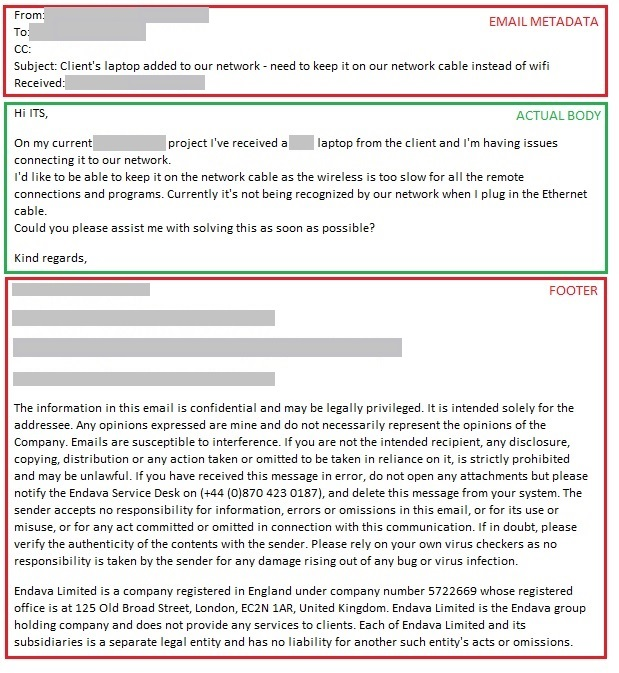
\includegraphics[width=0.65\textwidth]{x}
        \end{figure}

        Podemos intentar ver como esta conformado este dataset, siendo para nosotros importantes los campos de $body$ y $urgency$.
        \begin{figure}[h!]
            \centering
            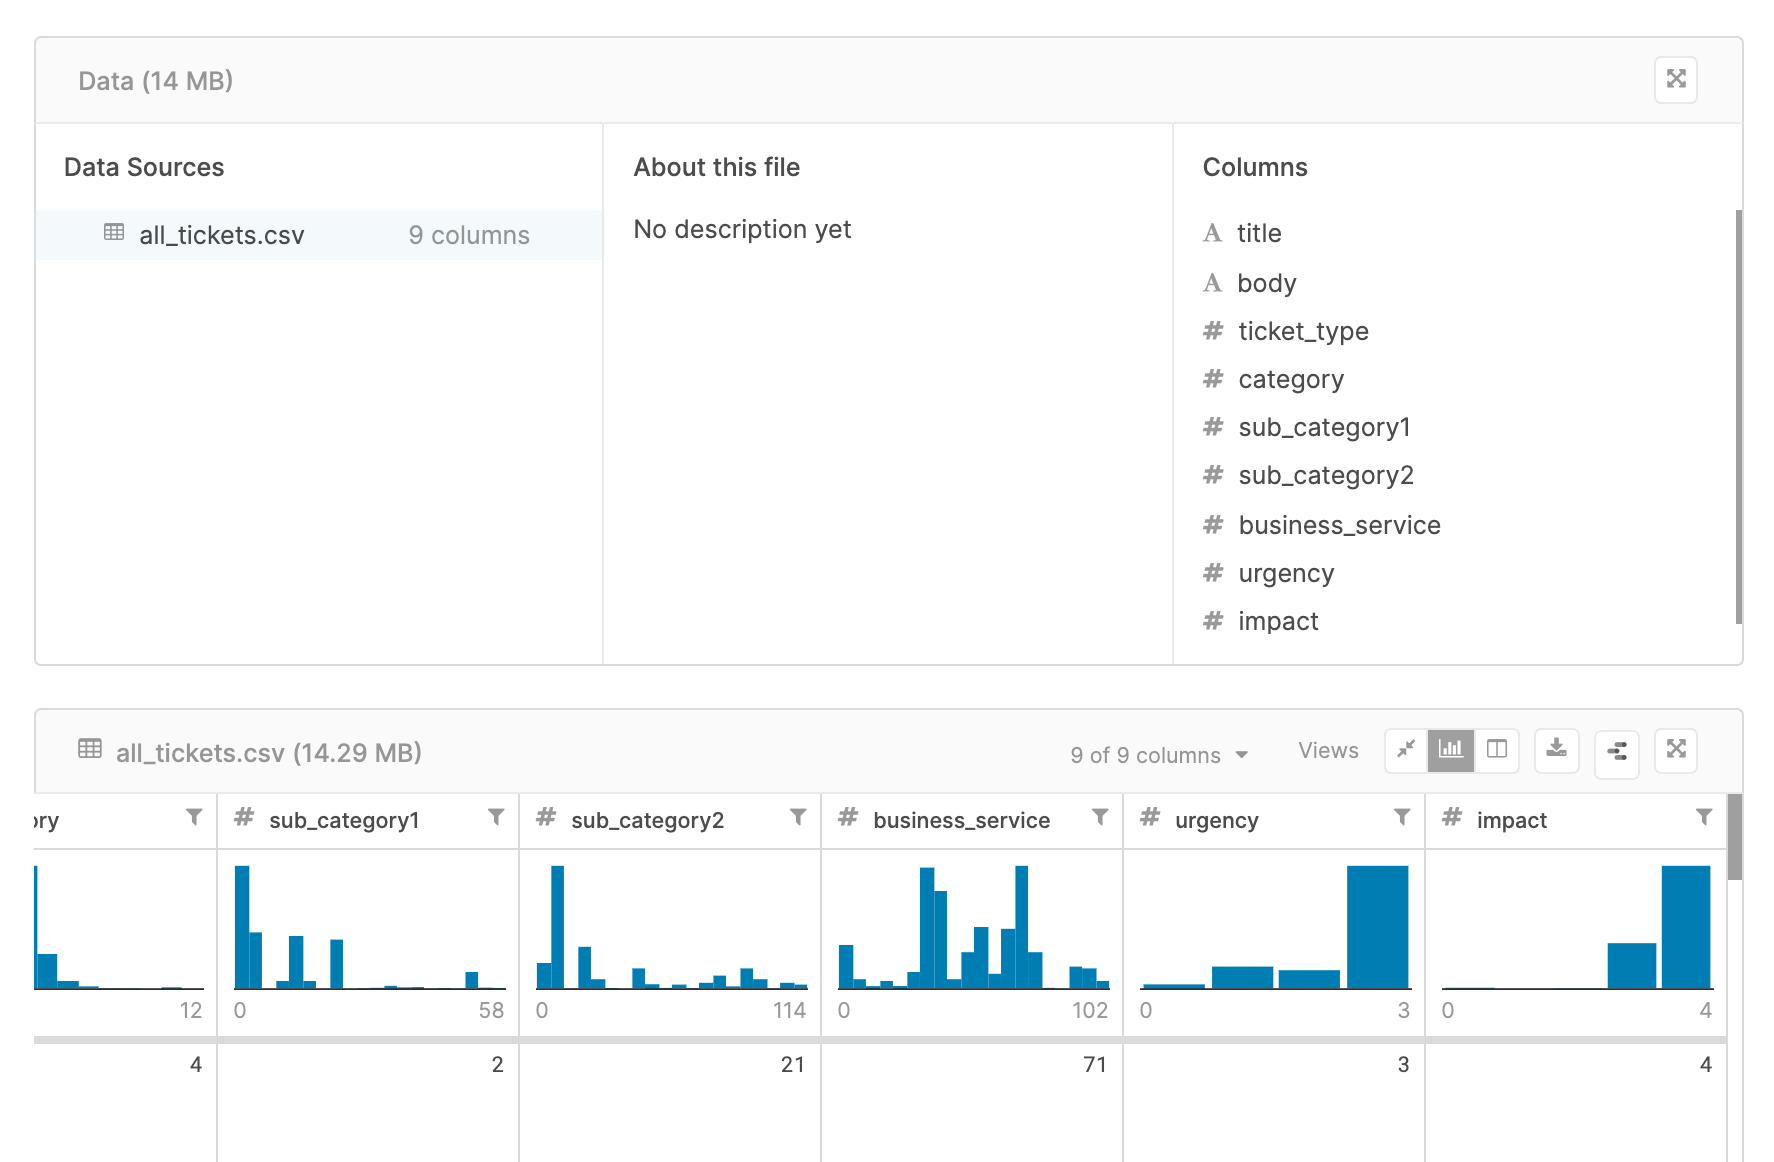
\includegraphics[width=0.65\textwidth]{x2}
        \end{figure}

        Ademas es importante notar que el campo de urgencia tiene solo 4 niveles, siendo por ejemplo el nivel 3 considera \Quote{low}.

    \chapter{La propuesta}
        Mi hipotesis sería que usando este dataset y 
        mediante aprendizaje supervisado (árboles de decisión) se podría crear un sistema que fuera capaz de clasificar con
        un gran alto nivel de exactitud (accuracy) (alrededor de un 85\%).

        Los árboles de decisión fueron elegidos por los puntos anteriormente dichos, sobretodo por la gran capacidad que interpretabilidad
        y que es conocido que los árboles de decisión tienen un gran rendimiento en el analisis de textos.

        En especial y debido a lo visto en clase se usara el J48 como clasificador.
        Tambien hablando mas detalladamente de el espacio de hipotesis tenemos que:
        \begin{itemize}
            \item Realiza aprendizaje por lote, que procesa todo el entrenamiento
            a la vez en lugar de aprendizaje incremental
            que actualiza una hipótesis después de cada ejemplo.
            \item Encuentra una sola hipótesis discreta.
        \end{itemize}

        La principal desventaja de esta propuesta es que se va a usar stringWordToVector, lo que perderemos una gran cantidad
        de información, sobretodo del contexto, pues nos quedaremos con un vector de frecuencias (o de existencia)
        pero no hay forma de saber donde estaban esas palabras originalmente en el texto, esta información para este
        problema puede llevar a que el sistema no se desempeñe tan bien como debería.

    \chapter{La implementación}

        \subsection{Preparación de los datos}

        Lo primero que tuvimos que hacer fue preparar los datos, el primer paso fue descargar el csv (all\_tickets.csv) y abrirlo con weka para crear
        un archivo arff que pudieramos usar desde Java, ahora si, con ese archivo listo (all\_tickets.arff).

        \begin{figure}[h!]
            \centering
            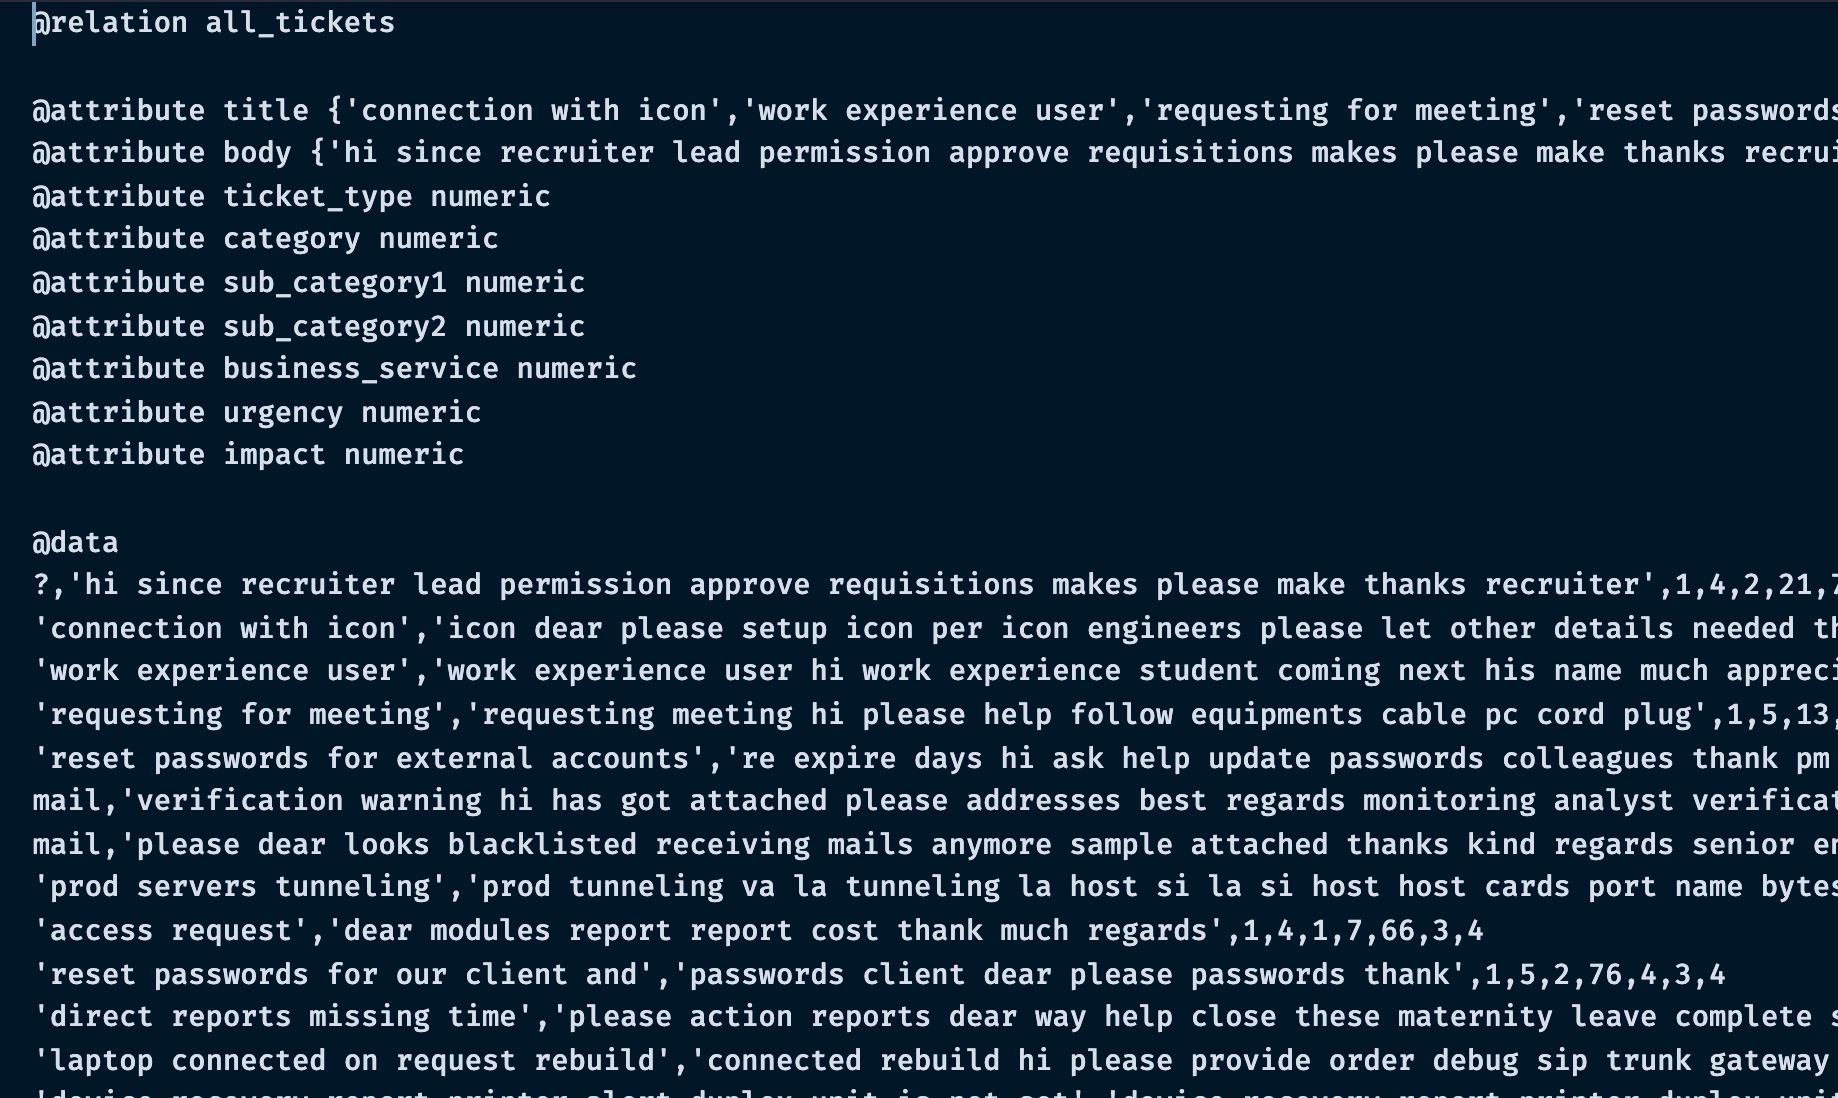
\includegraphics[width=0.65\textwidth]{ff}
        \end{figure}

        Ahora, lo siguiente fue quedarnos solo con los campos que necesitamos, en este caso el body y la etiqueta, por lo que eliminamos
        todos los demas.

        Ahora, tuvimos que usar dos filtros de weka para podemos poner los datos con los tipos apropiados.
        Primeramente tuvimos que usar el $NumericToNominal$ para poder poner las etiquetas como un dato nominal y no numerico.

        después tuvimos que hacer algo similar con el body que por defecto weka lo tomaba como un dato nominal.

        Ahora con ambos datos del tipo correcto ya podiamos usar $StringToWordVector$, a este tuvimos que darles varios parametros
        especiales (con la ayuda de $splitOptions$), en especial buscamos reducir la cantidad de palabras a conservar, pasando 
        de 1000 a ~100, decidimos dejar la diferencia entre mayusculas y minisculas y tambien no usar un steamer pues no existe una
        compatibilidad total (ademas de que diferentes experimentos demostraron que su uso no afectaba significativamente el desempeño del
        ente), con est filtro aplicado, ahora si estabamos listo para clasificar, teniendo alrededor de 101 atributos.


        \subsection{Creación del clasificador}

        Esto fue mucho mas sencillo e igualmente buscamos crear el modelo mas sencillo que fuera capaz de resolver el problema, llegando
        a que el parametro que mas afectba el desempeño del sistema era la cantidad de elementos necesario para crear una hoja,
        un valor de 15 resulto ser mucho mas efectivo en reducir el tamaño del arbol y aumentar el desempeño.

        Ahora tambien fue importante cambiar el tamaño del bache a 64, siendo una creencia común que conocía y comprobé que usar 
        una potencia de 2 aumenta significativamente el tiempo de entrenamiento.

        \subsection{Evaluación}

        Lo que hicimos para evaluar al sistema fue partir nuestros datos, elegimos un 80\%, algo muy importante (y que me tomo dos horas
        darme cuenta y cambio el resultado del sistema de un 40\% a un 85\%) es que antes de partir los datos lso \Quote{revolvimos},
        para evitar que cierto grupo de etiquetas quedara sobrerepresentado en algun conjunto.

        \subsection{interpretación}

        Con esto listo creamos un evaluador y medimos el resultado de nuestro clasificador.
        \begin{figure}[h!]
            \centering
            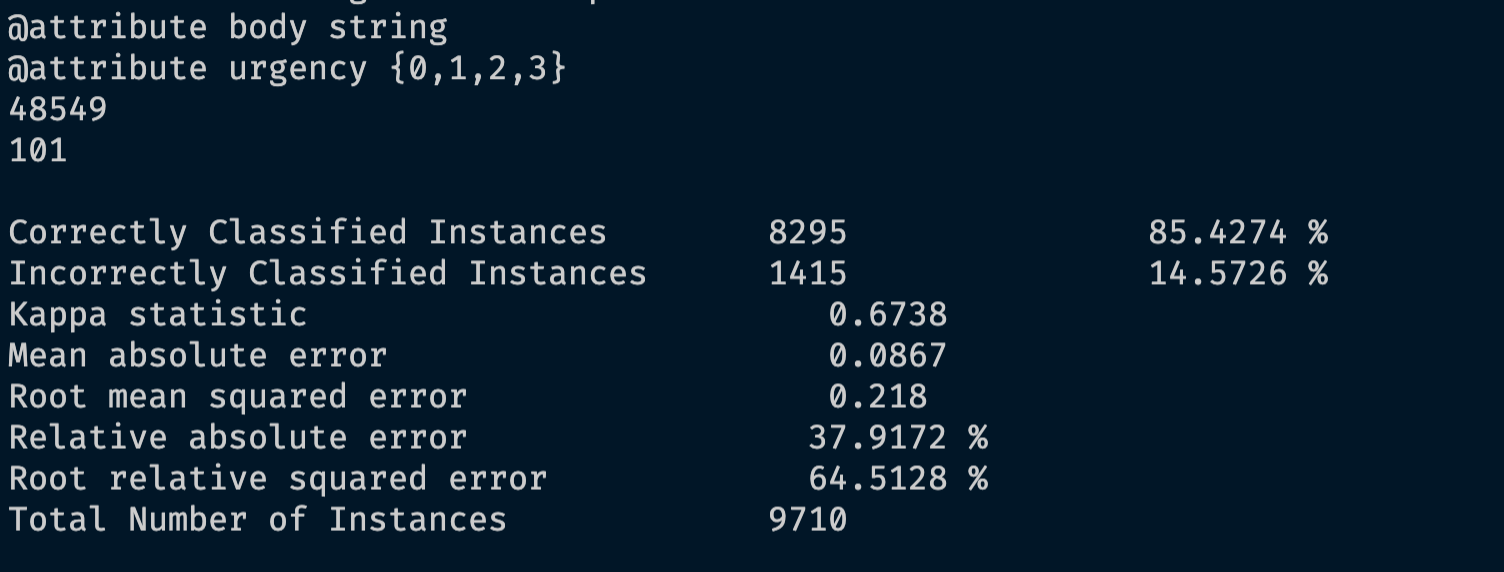
\includegraphics[width=0.65\textwidth]{result}
        \end{figure}

        En este podemos ver inmediatamente que nuestro sistema cumplio nuestro objetivo, 
        logran un mas de 85\% de accuracy en el conjunto de prueba.

        Ademas viendo a la matriz de confusión vemos que los errores se distribuyen de manera informe.
        Finalmente y como una posible forma de llevarlo a las manos de los usuarios cree un programa que usa
        los modelos y al que tu le pasas un texto por la terminal y te regresa su nivel estimado de urgencia.

        \begin{figure}[h!]
            \centering
            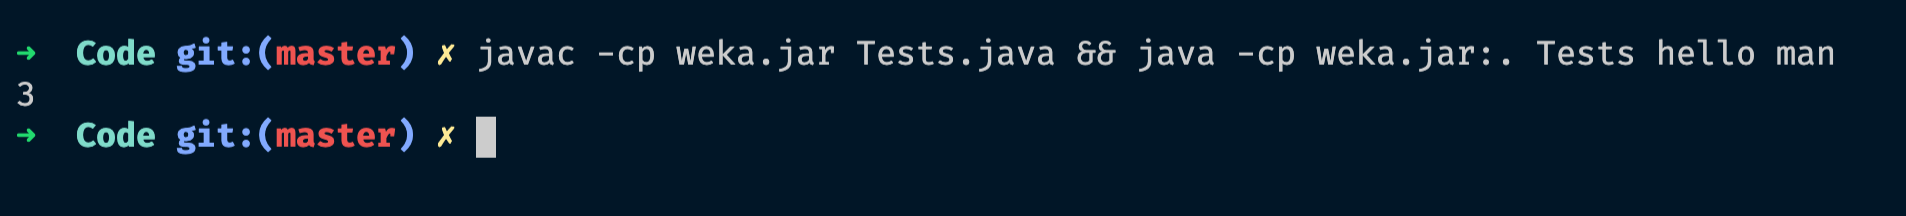
\includegraphics[width=0.65\textwidth]{man}
        \end{figure}

        \subsection{Codigo}
        \subsubsection{Codigo principal}
        Compilarse usando: javac -cp weka.jar Project.java \&\& java -cp weka.jar:. Project   
        y java v13
        \lstinputlisting[language=Java, gobble=6]{../Code/Project.java}

        \subsubsection{Codigo de pruebas del usuario final}
        \begin{figure}[h!]
            \centering
            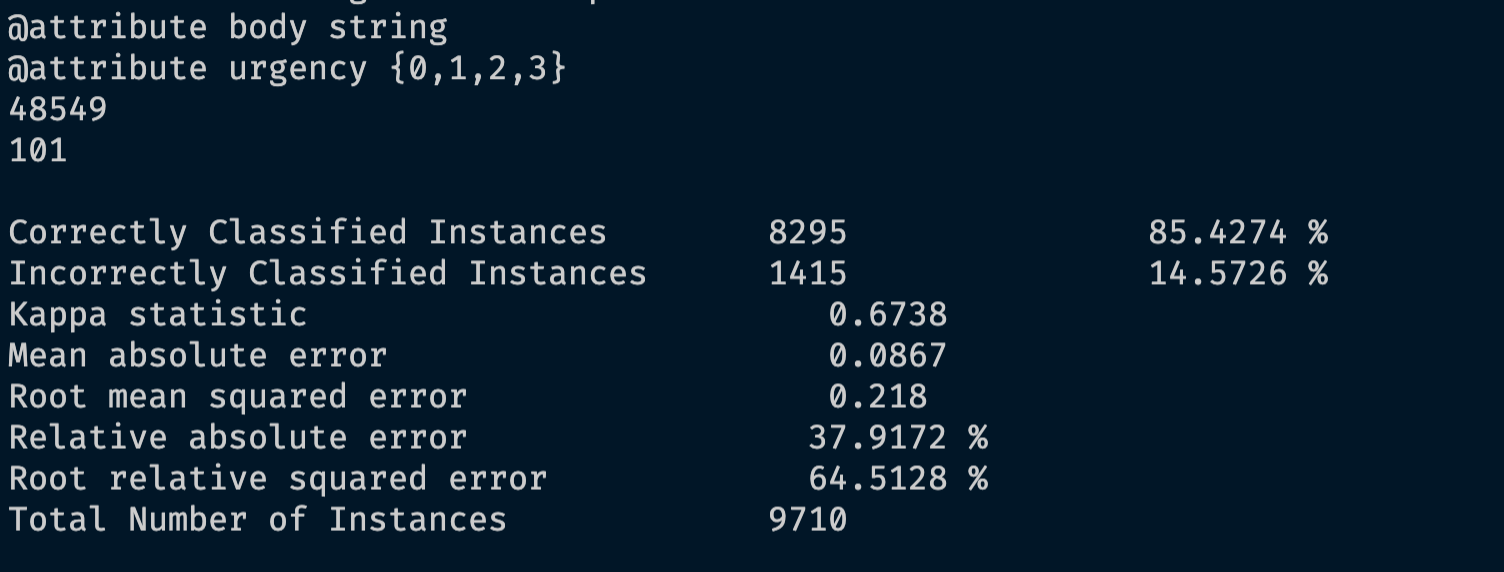
\includegraphics[width=0.65\textwidth]{result}
        \end{figure}
        \lstinputlisting[language=Java, gobble=6]{../Code/Tests.java}



        \subsection{Posibles mejoras a futuro}

            \begin{itemize}
                \item Por un lado seria interesante ver como usando $IDFTransform/TFTransform$
                podriamos alterar los resultados.
                \item Debido a que los datos no estan balanceados usar el accuracy no es la mejor
                idea y se debe hacer con cuidado.
            \end{itemize}

        \subsection{Conclusión}

        Gracias a los resultados vimos que es posible crear un algoritmo con la ayuda de los árboles de decisión
        que nos permite clasificar con un gran desempeño la urgencia de un \Quote{support ticket}.



\begin{thebibliography}{10}

  \bibitem{1} 
      \textit{Aidan Wilson}, 
      Sep 29, 2019 \\
      \url{https://towardsdatascience.com/a-brief-introduction-to-supervised-learning}

  \bibitem{2} 
      \textit{Diego Lopez Yse}, 
      Apr 17, 2019 \\
      \url{https://towardsdatascience.com/the-complete-guide-to-decision-trees}


\end{thebibliography}



\end{document}